\documentclass{article}
\usepackage[utf8]{inputenc}
\usepackage{graphicx}
\usepackage[left=25mm,top=10mm,right=25mm,bottom=5mm]{geometry}
\usepackage{amsmath}
\usepackage{array}

\title{\Huge \textbf{AE 238 Assignment 2}}
\author{\Huge \textbf{Krishna Wadhwani - 160010031 }}
\date{January 2018}


\begin{document}

\maketitle


\noindent \title{\LARGE \textbf{Question 1}}
\bigbreak

    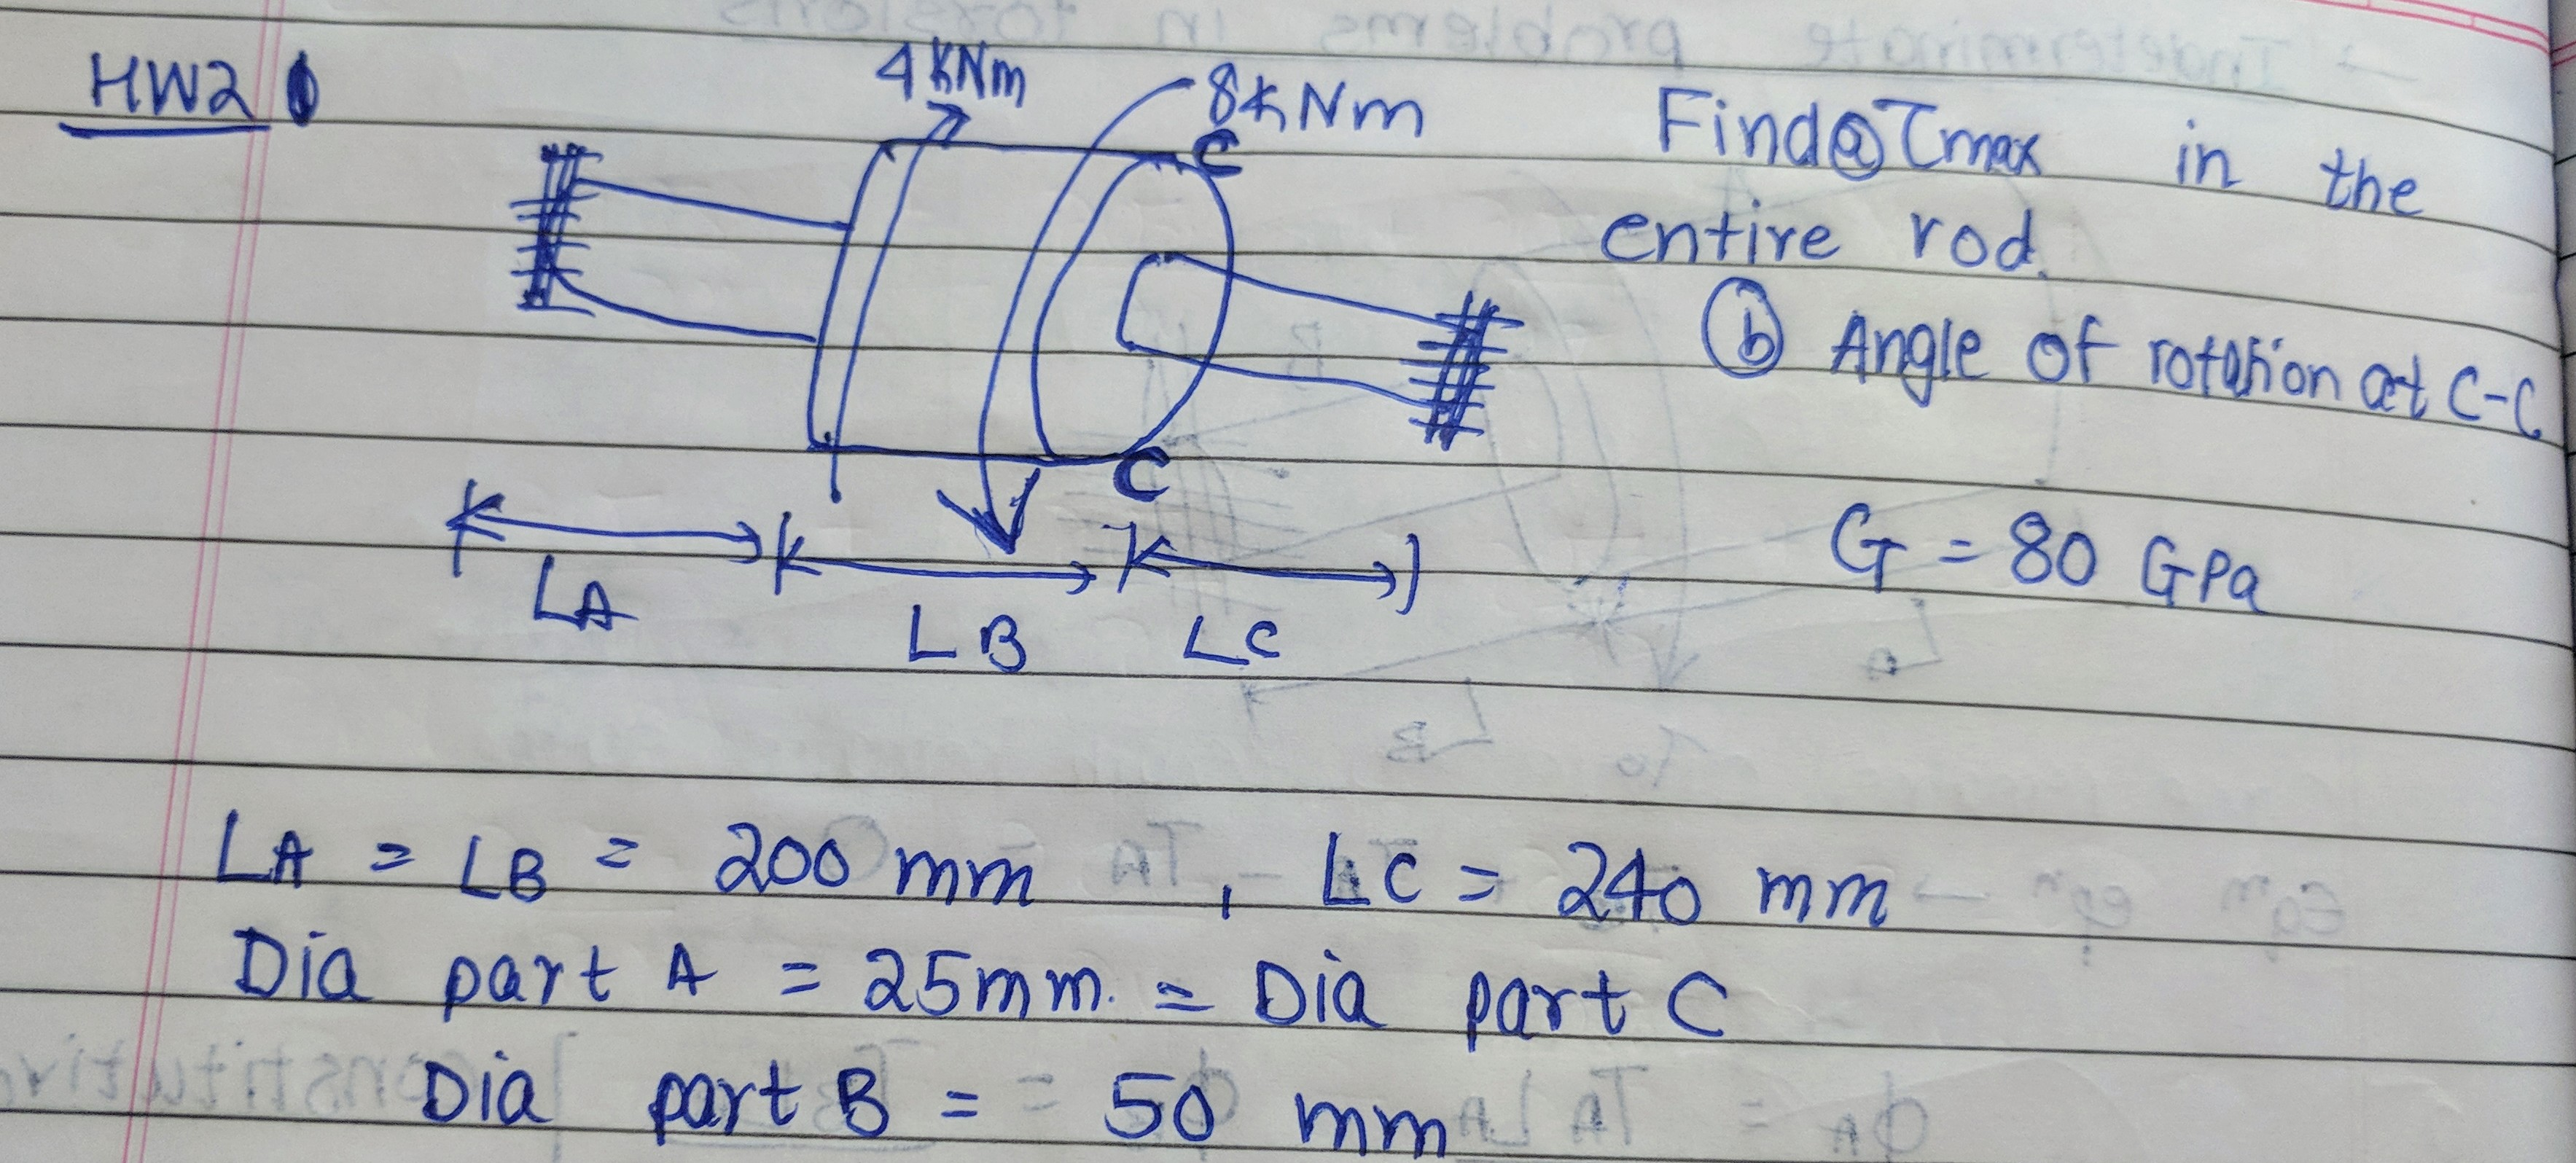
\includegraphics[scale=0.1]{AE238_A2Q.jpg}
\bigbreak
\noindent \underline{Notation used}: 
\begin{itemize}
\item $T_A$ and $T_C$ denote the restoring moment developed at the clamped ends in regions A and C respectively, whereas $T^A$, $T^B$ and $T^C$ denote the moments in region A, B and C respectively.
\item $T_A$ is assumed in clockwise direction whereas $T_C$ is assumed in counter-clockwise direction
\item $\phi_A, \phi_B$ and $\phi_C$ denote angle of rotation in regions A, B and C respectively and $\phi_{CC'}$ denotes angle of rotation at C-C'.
\item Counter-clockwise moment is considered positive.
\end{itemize} 

\bigbreak
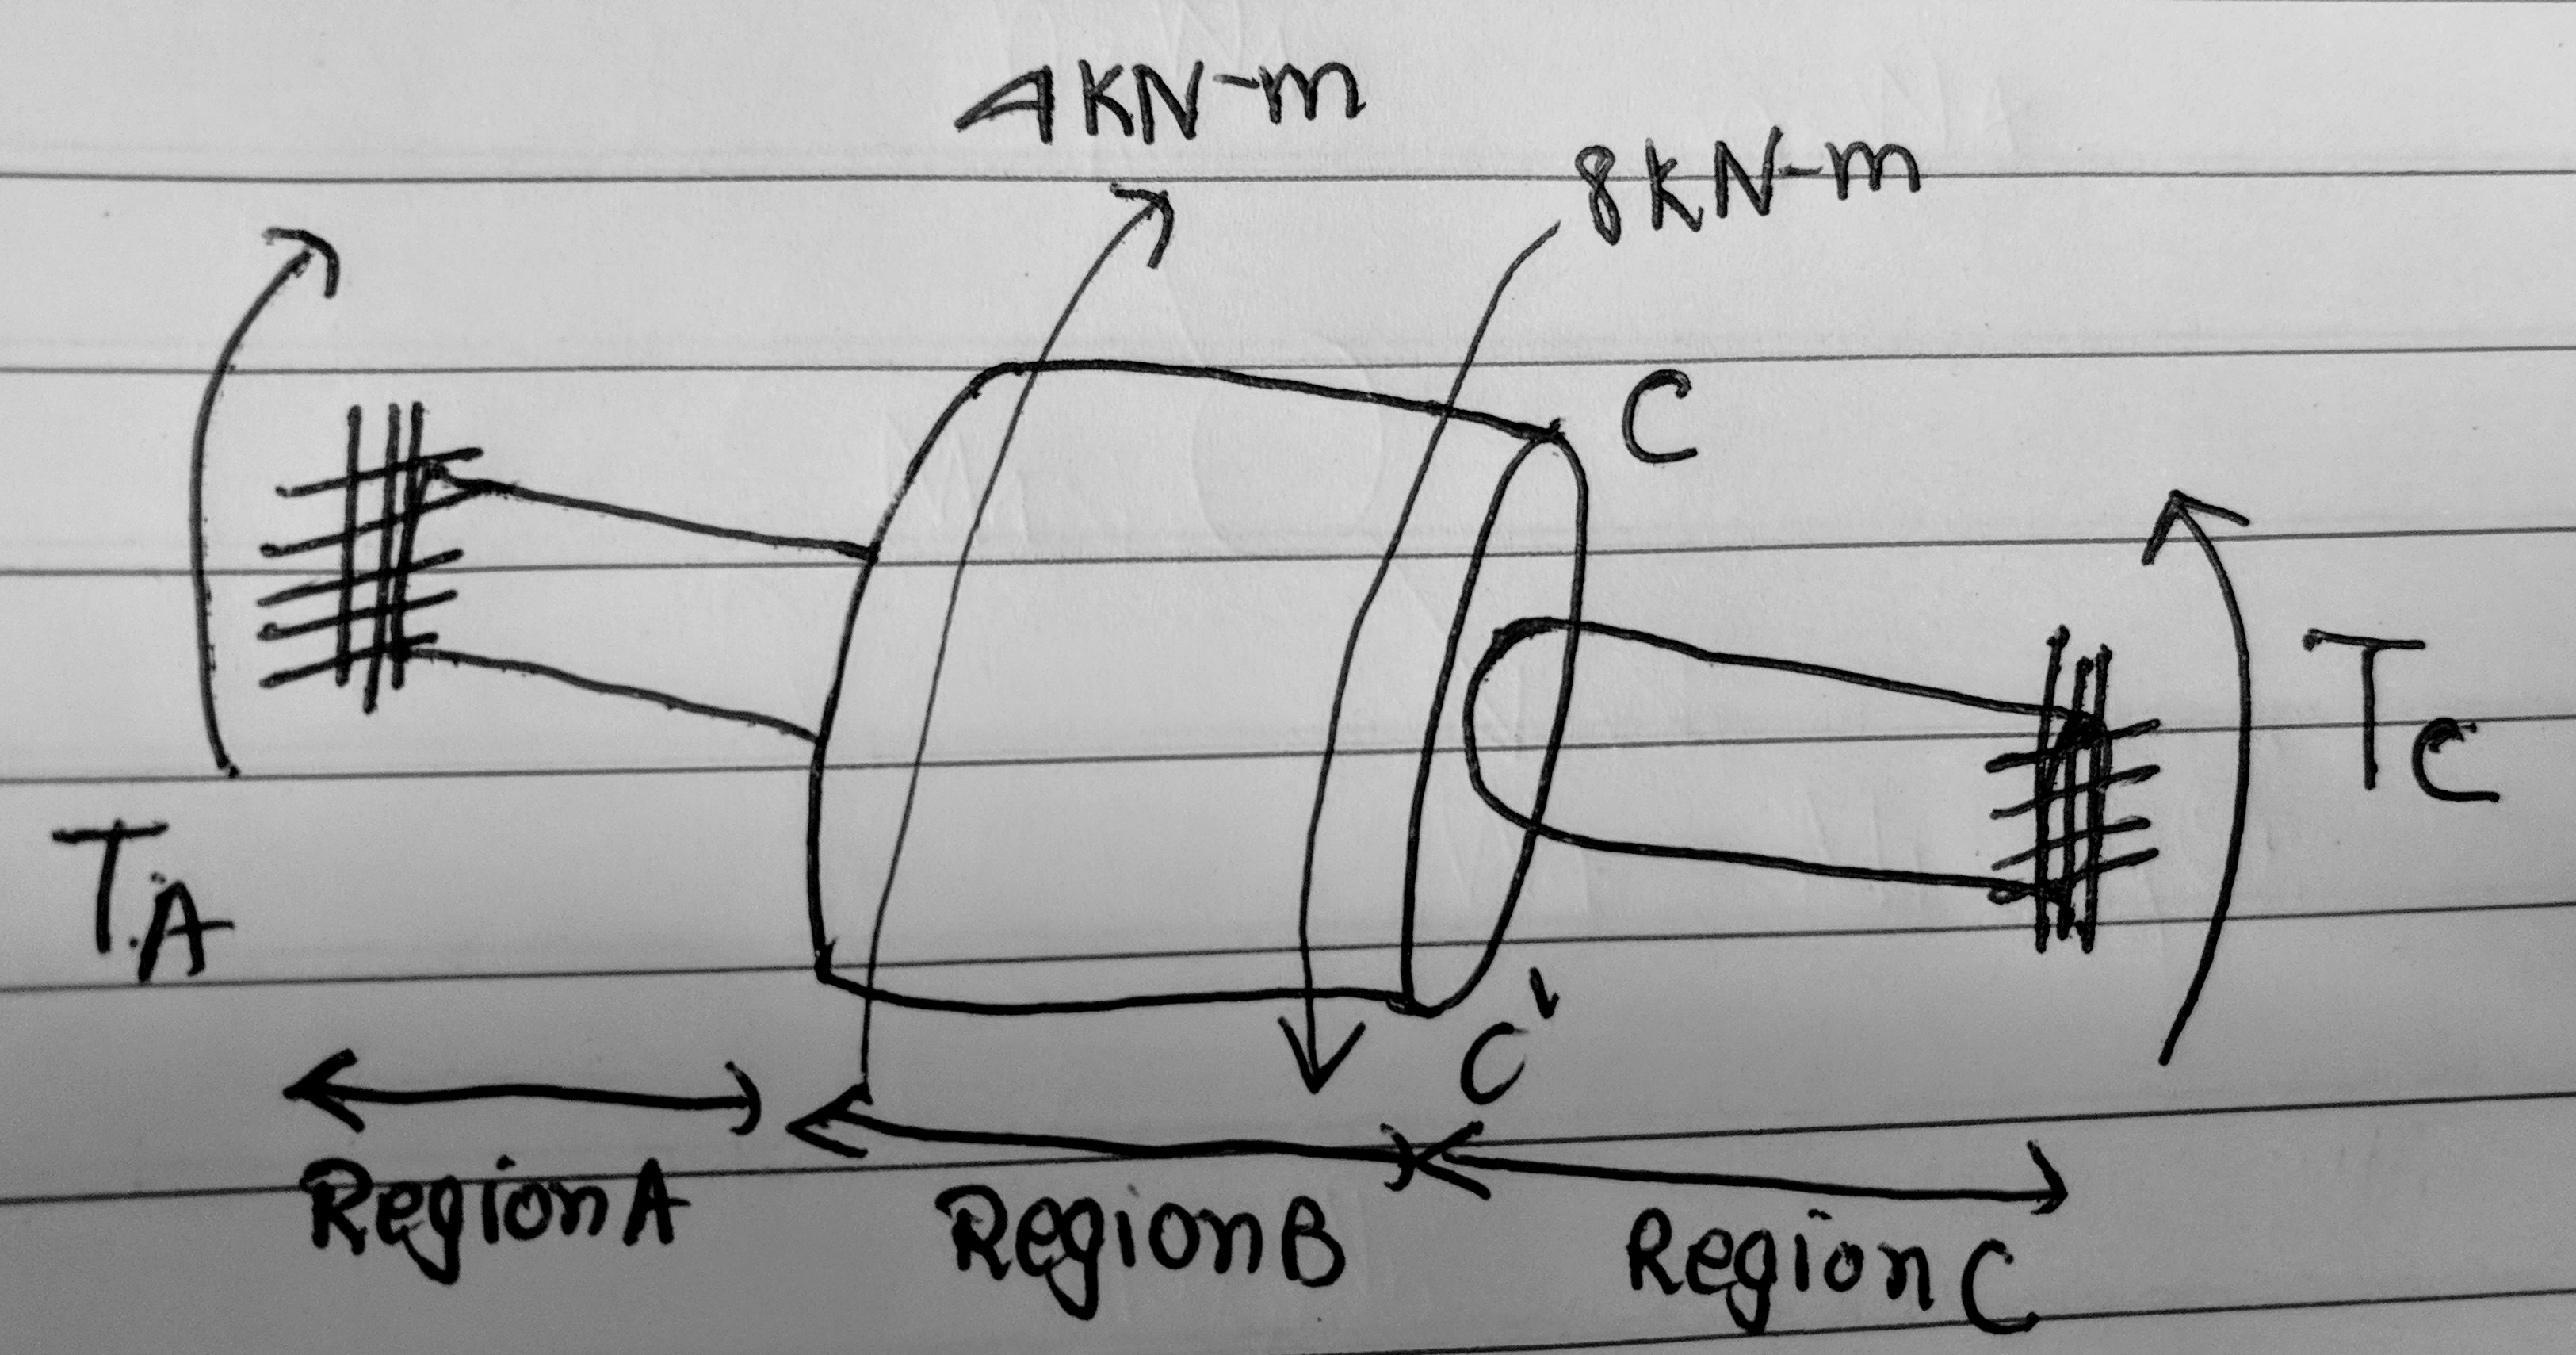
\includegraphics[scale=0.075]{1.jpg}

\noindent \underline{Moment equilibrium equation} for the entire structure: \\
$-T_A-4+8+T_C=0$\\
$\implies -T_A+T_C+4=0$\\

\noindent \underline{Compatibility equation} (As the structure is clamped at both ends, total rotation will be 0): \\
$\phi_A+\phi_B+\phi_C=0$\\
From \underline{constitutive relations}: 
$\phi= \dfrac{TL}{GJ}$\\
$\implies \dfrac{T^AL_A}{GJ_A}+ \dfrac{T^BL_B}{GJ_B}+ \dfrac{T^CL_C}{GJ_C}=0$\\

\noindent Now from the above figure, we can see that $T_A- 4 + T_B = 0 $\\

\bigbreak
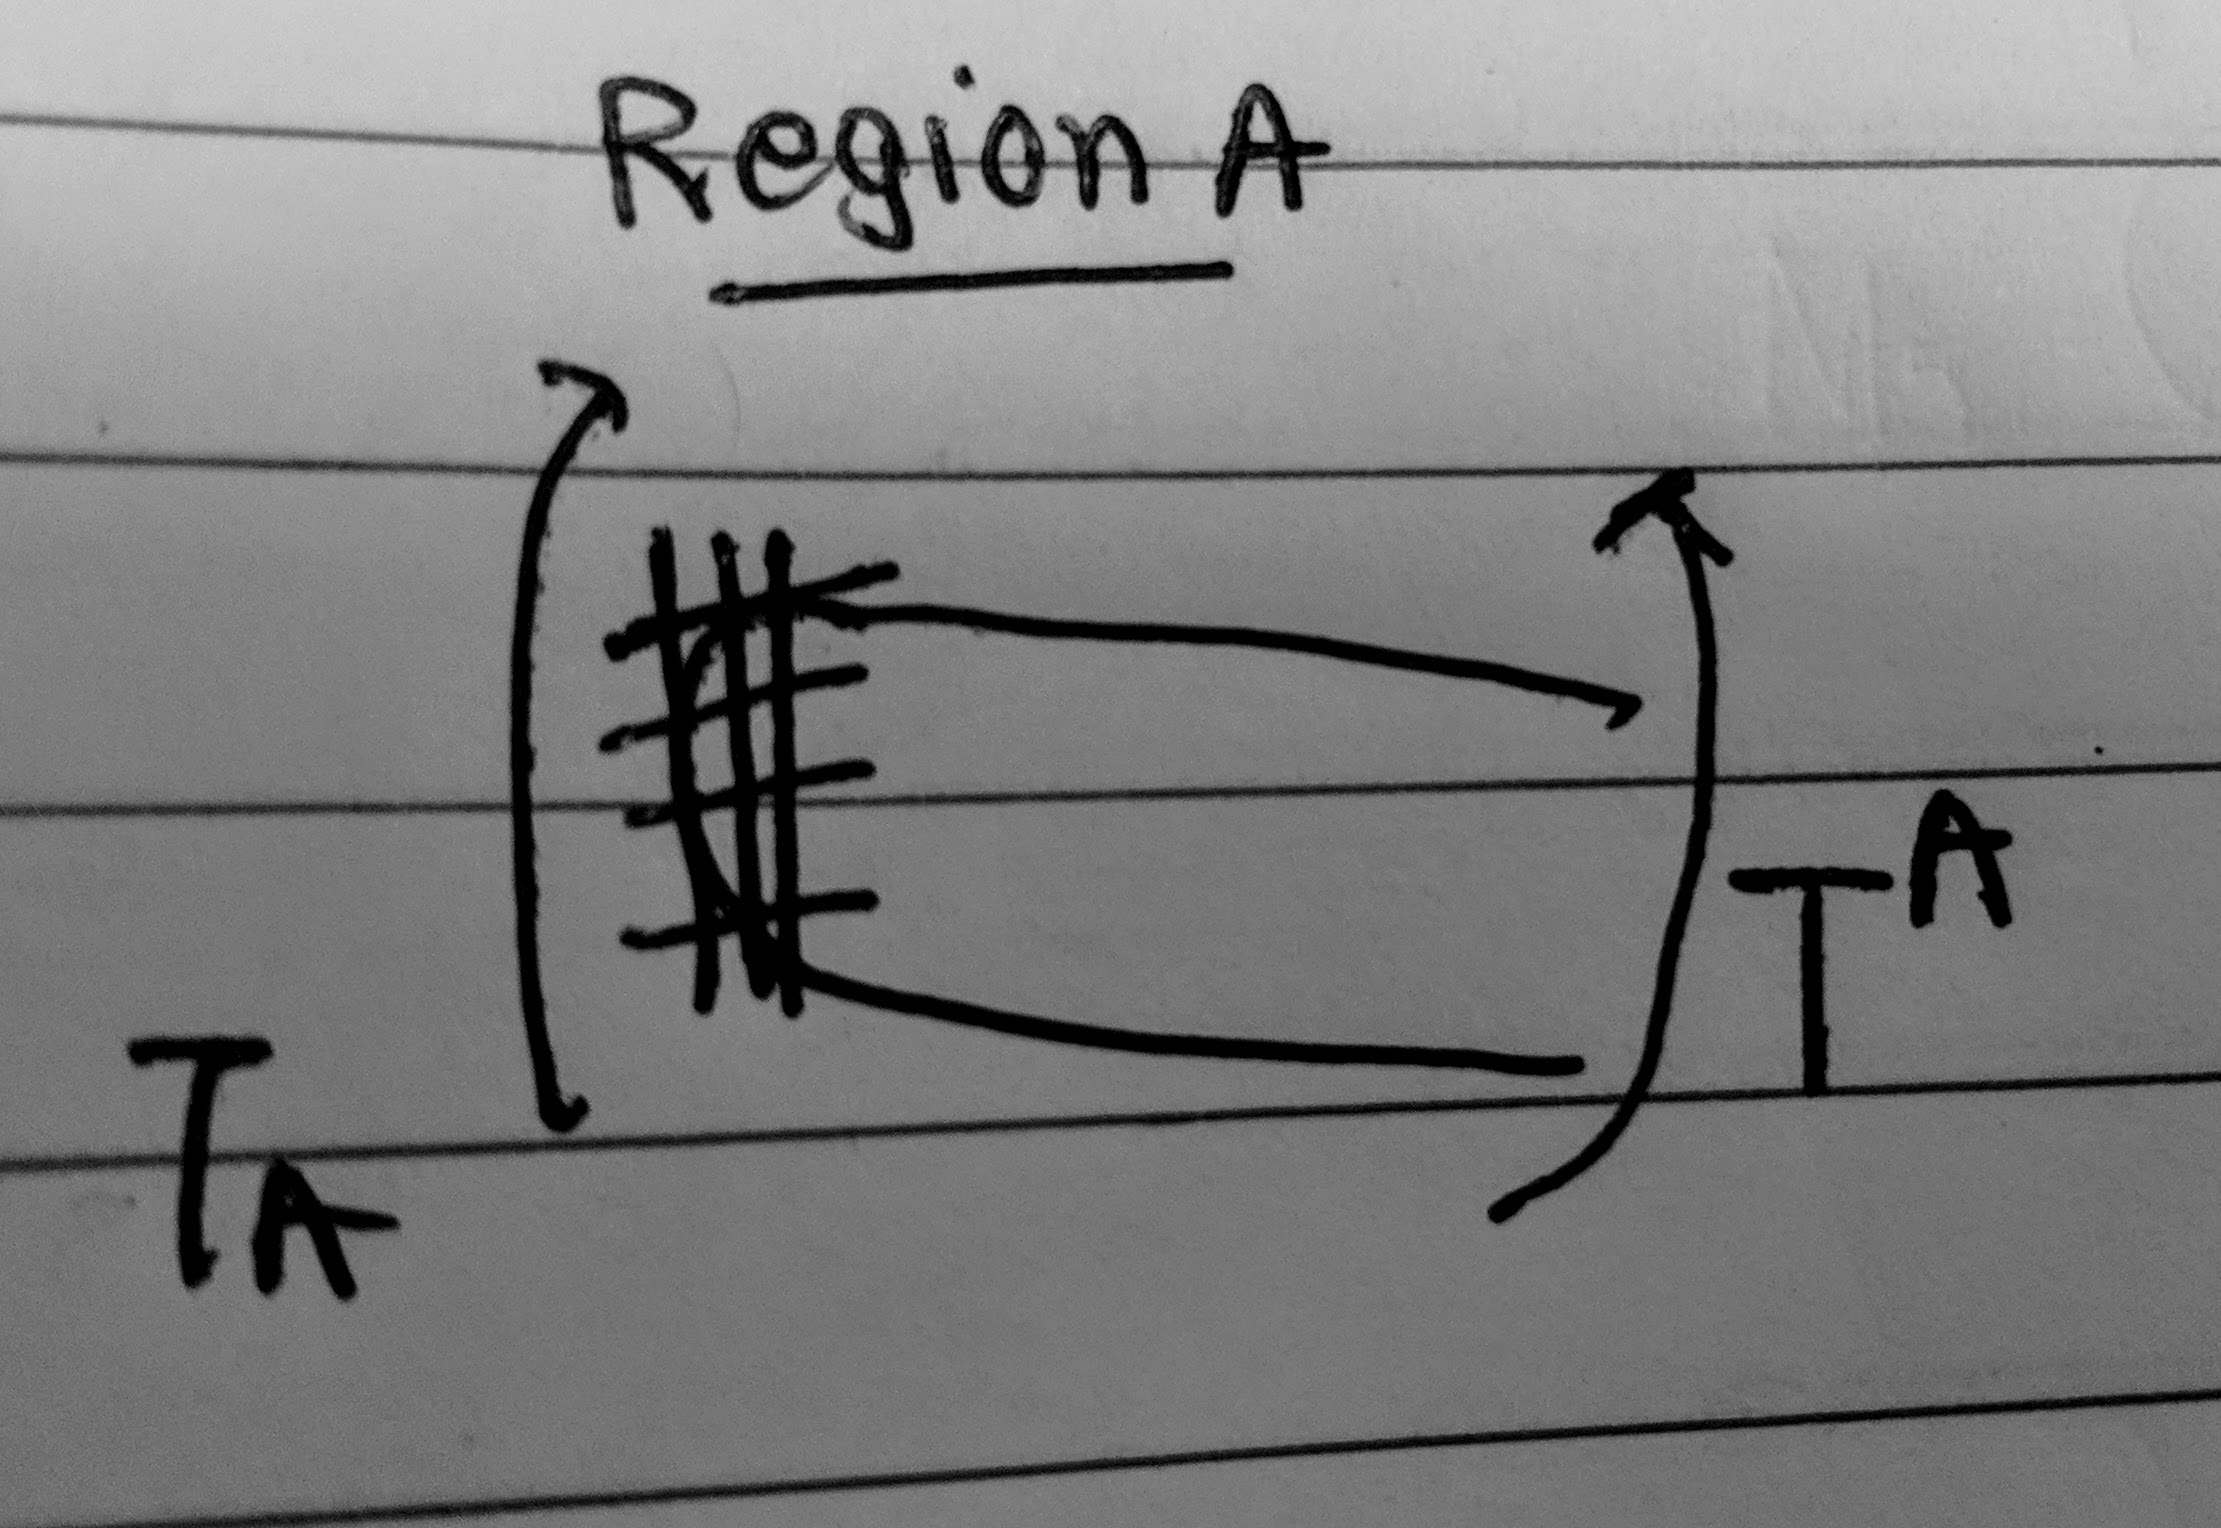
\includegraphics[scale=0.05]{A.jpg} 

\bigbreak
\noindent $-T_A+T^A=0$\\
$\implies T^A=T_A$\\

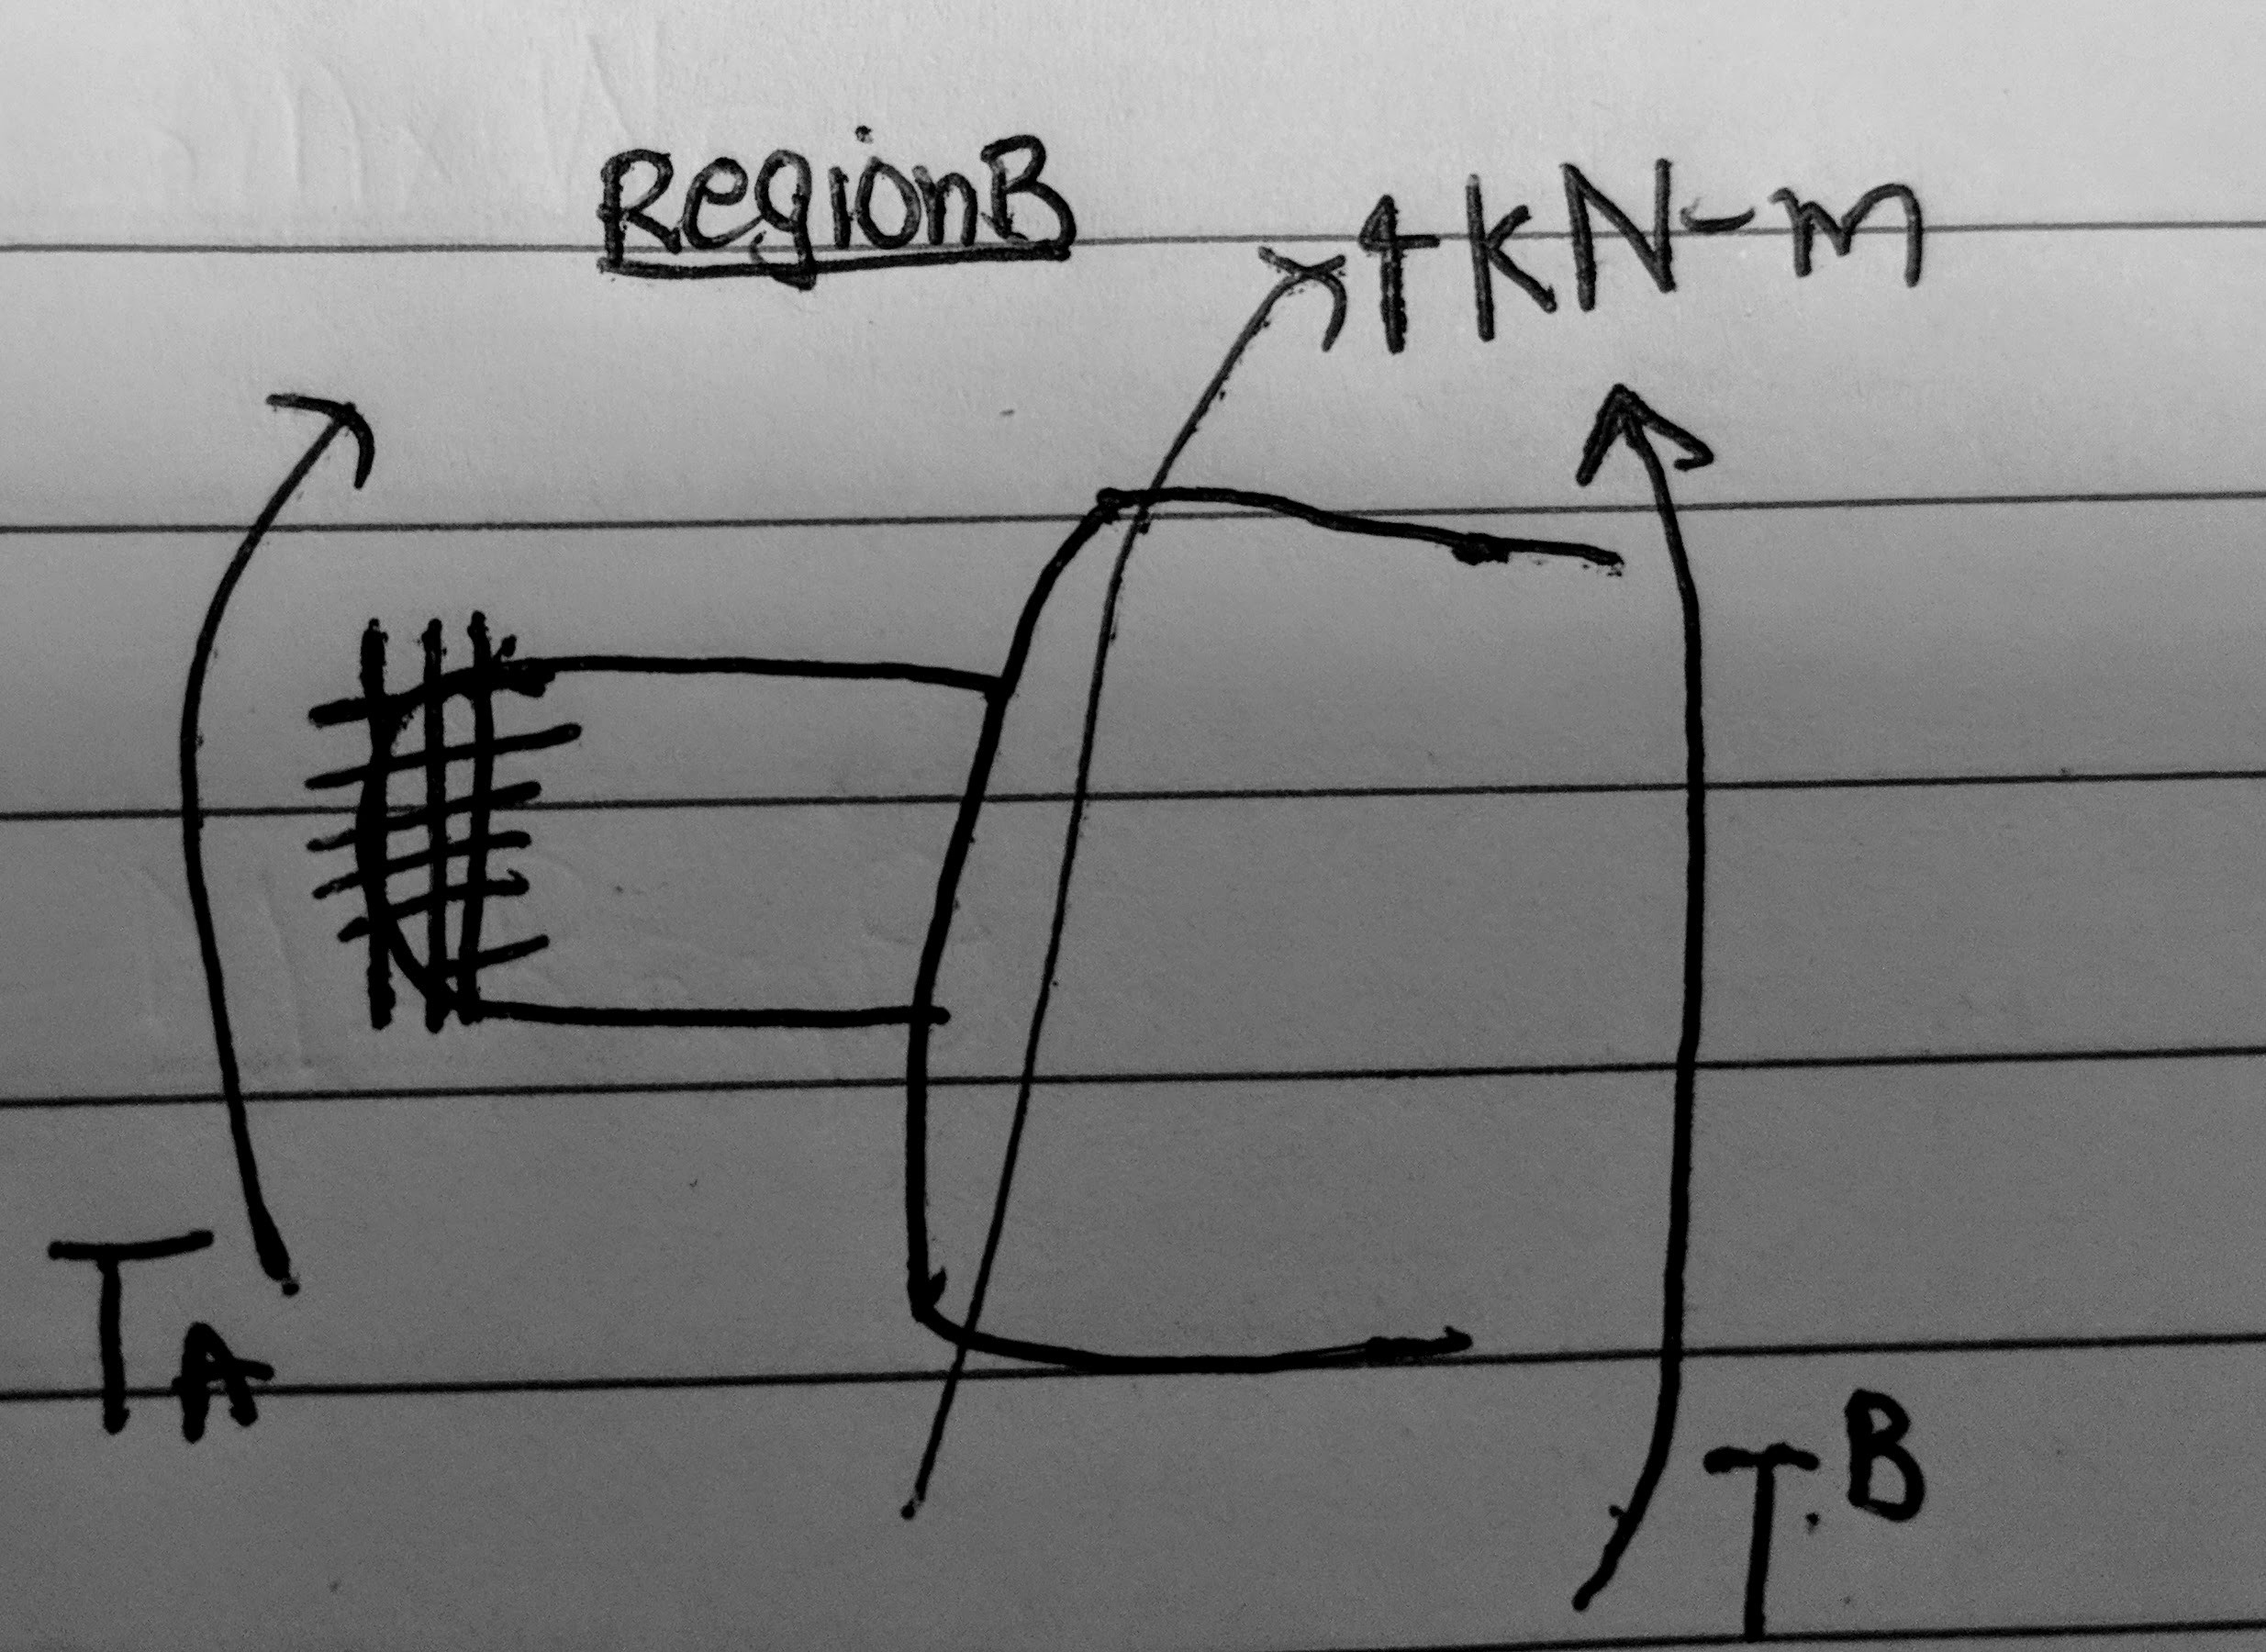
\includegraphics[scale=0.05]{B.jpg}

\bigbreak
\noindent $ -T_A-4+T^B=0$\\
$\implies T^B=T_A+4$\\

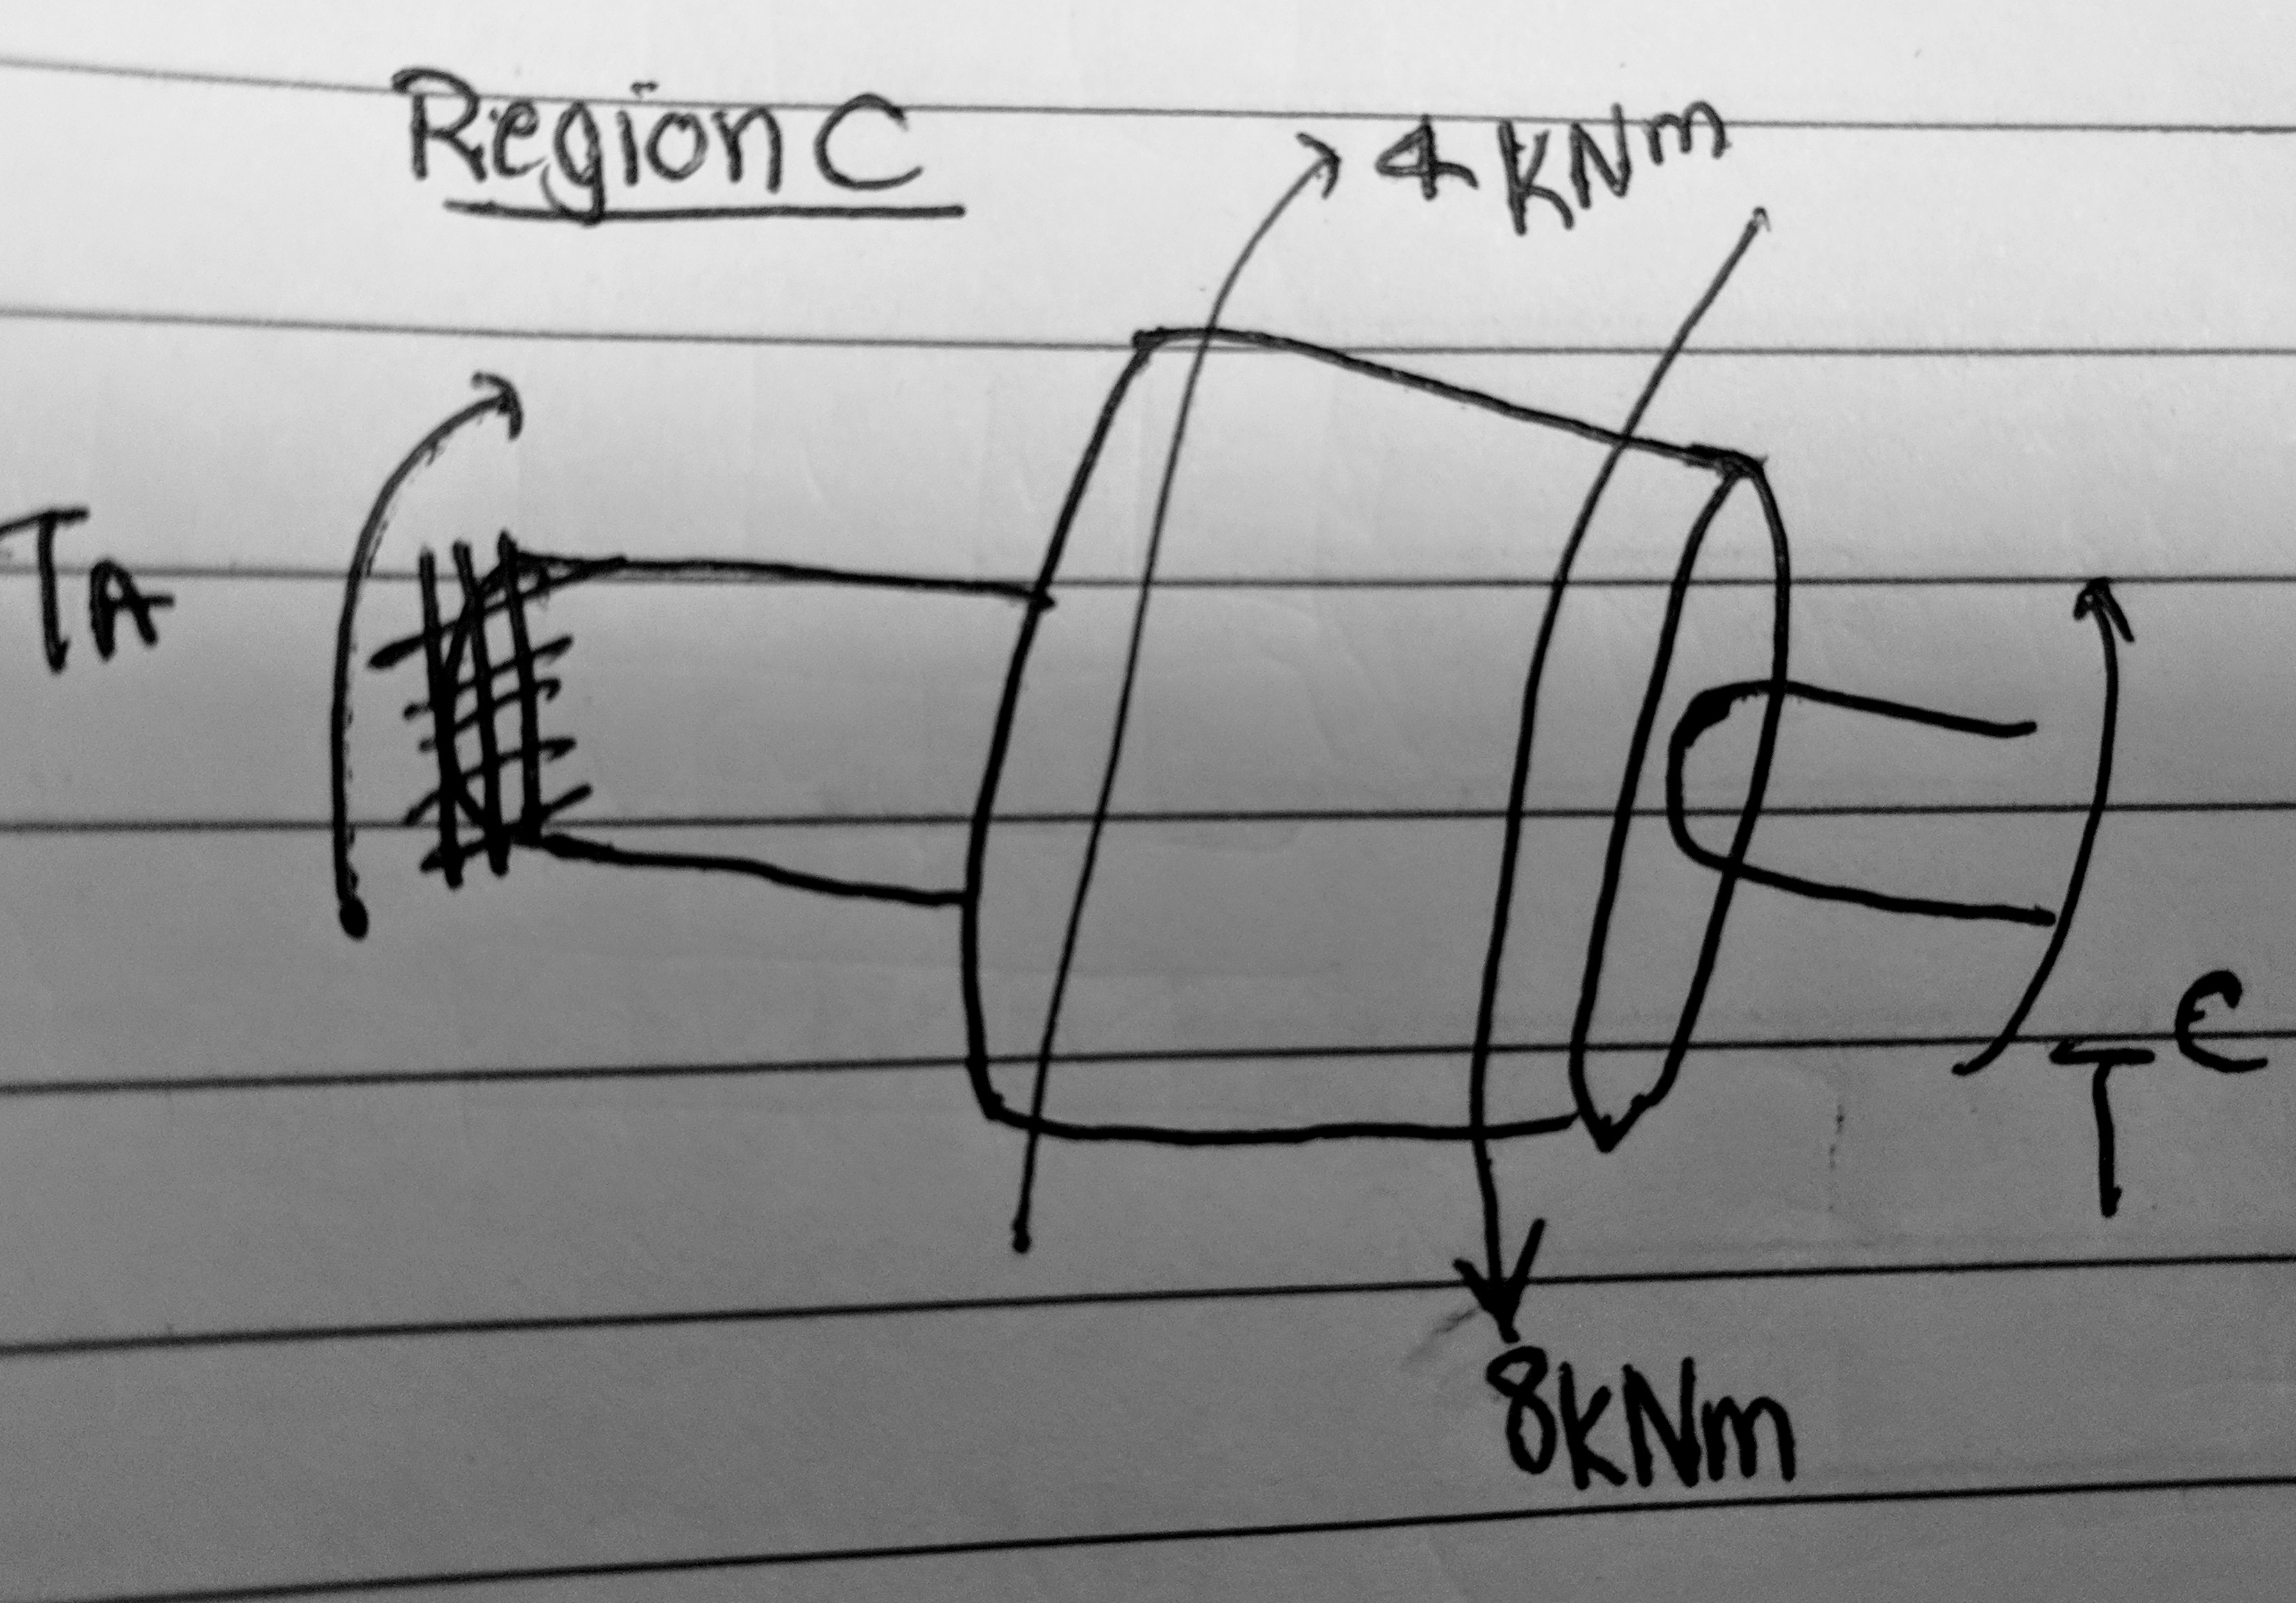
\includegraphics[scale=0.05]{C.jpg}

\bigbreak
\noindent $- T_A-4+8+T^C=0$\\
$\implies T^C=T_A-4$\\

\noindent $\implies \dfrac{T_AL_A}{GJ_A}+ \dfrac{(T_A+4)L_B}{GJ_B}+ \dfrac{(T_A-4)L_C}{GJ_C}=0 $\\


\noindent Now we will substitute the values as per the information given in the question:\\
Given:\\ $L_A=200mm, L_B=200mm, L_C=240mm $\\
$G= 80GPa$\\
$2R_A =25mm, 2R_B= 50mm, 2R_C= 25mm$\\
As $J= \dfrac{\pi R^4}{2}$: \\
$J_A= \dfrac{\pi R_A^4}{2}, J_B= \dfrac{\pi R_B^4}{2}, J_C= \dfrac{\pi R_C^4}{2}$\\
$\implies J_A= 3.835 \times 10^{-8} m^4$\\
$\implies J_B= 6.136 \times 10^{-7} m^4$\\
$\implies J_C= 3.835 \times 10^{-8} m^4$\\

\noindent Substituting the above values, we get:\\
$6.519T_A+0.4017(4+T_A)+7.823(4+T_A)=0$\\
$13.9403T_A+32.8988=0$\\
$\implies T_A= 2.007 kN{\text -}m$\\

\noindent As $T_C= 4+T_A$\\
$\implies T_C= -1.993 kN{\text -}m$

\noindent Finding $\tau_{max}$ in each of the three parts of the rod A,B and C using the formula 
$\tau_{max}=\dfrac{TR}{J}$\\

\noindent $\tau_{max}^A=\dfrac{T^AR_A}{J_A}$\\
Here $T^A=T_A= 2.007 kN{\text -}m$\\
$\implies \tau_{max}^A=654.17 MPa$\\

\noindent $\tau_{max}^B=\dfrac{T^BR_B}{J_B}$\\
Here $T^B=T_A+4= 6.007 kN{\text -}m$\\
$\implies \tau_{max}^B=244.74 MPa$\\

\noindent $\tau_{max}^C=\dfrac{T^CR_C}{J_C}$\\
Here $T^C=T_A-4= 1.993 kN{\text -}m$ (Considering magnitude only) \\
$\implies \tau_{max}^C=649.61 MPa$\\

\noindent So, $\tau_{max}$ in the entire rod is 654.17 $MPa$ in region A. \\

\noindent \underline{For Angle of rotation}:\\

\noindent $\phi_A=\dfrac{T^AL_A}{GJ_A}$\\
$\implies \phi_A= \dfrac{(2.007 \times 10^3)(200 \times 10^{-3})}{(80 \times 10^9)(3.835 \times 10^{-8})}$\\
$\implies \phi_A=0.1308$ radians or $7.49^\circ$\\

\noindent $\phi_B=\dfrac{T^BL_B}{GJ_B}$\\
$\implies \phi_B= \dfrac{(6.007 \times 10^3)(200 \times 10^{-3})}{(80 \times 10^9)(6.136 \times 10^{-7})}$\\
$\implies \phi_B=0.024$ radians or $1.38^\circ$\\

$\phi_C=\dfrac{T^CL_C}{GJ_C}$\\
$\implies \phi_C= \dfrac{(-1.993 \times 10^3)(240 \times 10^{-3})}{(80 \times 10^9)(3.835 \times 10^{-8})}$\\
$\implies \phi_C=-0.1548$ radians or $-8.87^\circ$\\

\noindent So, Angle of rotation at C-C' interface $\phi_{CC'}=\phi_A+\phi_B$ \\
$\phi_{CC'}=-\phi_C$\\
$\phi_{CC'}= 8.87^\circ$ \\
\bigbreak

\begin{center}
\title{\LARGE \textbf{THE END}}
\end{center}
\end{document}
